\section{Experimental Results}
\label{experiment}

\subsection{Dataset}
\label{experiment:dataset}
We experiment on four trajectories datasets provided by \cite{ijcai15} that were
extracted from Yahoo! Flickr Creative Commons 100M (a.k.a. YFCC100M) dataset\cite{yfcc100m} 
using photos and videos with geographical locations, timestamps, user identifications etc,
and another trajectories dataset using photos in YFCC100M that were taken in Melbourne,
trajectories were extracted the same way as that described in \cite{ht10, ijcai15},
the time that a user arrived a POI was approximated by the time the first photo taken by that user at that POI,
similarly, the time that a user leaved a POI was approximated by the time the last photo taken by that user at 
that POI \cite{ijcai15}.
An example of trajectory in Toronto dataset was shown in figure \ref{fig:traj}, 
%TODO: explain what is a POI/photo in the figure
and statistics of the five datasets are described in table \ref{table:data}.


\begin{figure}
\centering
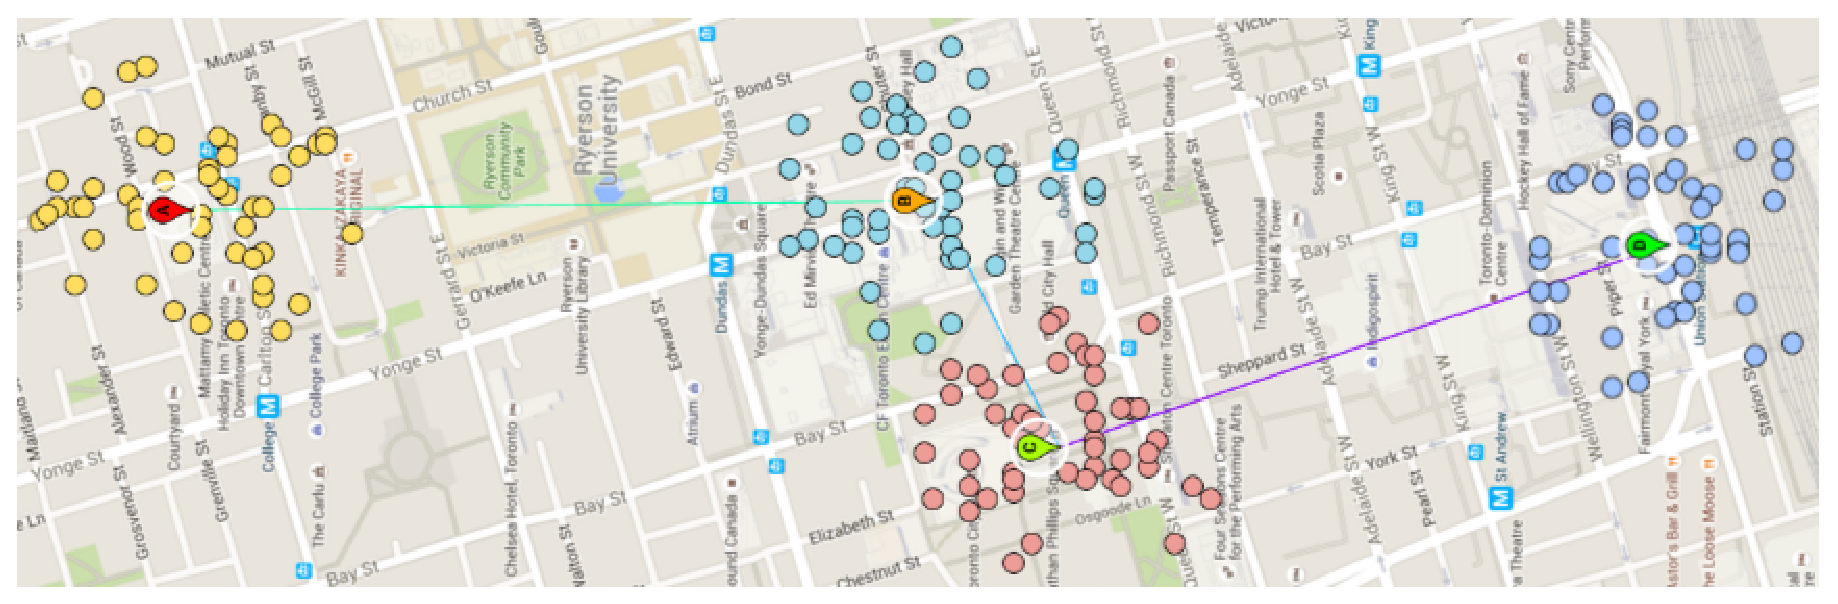
\epsfig{file=traj_eg.eps, width=3.5in}
\caption{An example of trajectory}
\label{fig:traj}
\end{figure}

\begin{table*}
\centering
\begin{tabular}{lrrrrr} \hline
\textbf{Dataset} & \textbf{\#Photos} & \textbf{\#POI Visits} & \textbf{\#Trajectories} & \textbf{\#Users} \\ \hline
Edinburgh & 82,060 & 33,944 & 5,028 & 1,454 \\ 
Glasgow & 29,019 & 11,434 & 2,227 & 601 \\ 
Osaka & 392,420 & 7,747 & 1,115 & 450 \\ 
Toronto & 157,505 & 39,419 & 6,057 & 1,395 \\ 
\hline
\end{tabular}
\caption{Statistics of trajectory dataset}
\label{table:data}
\end{table*}


\subsection{Evaluation Metrics}
\label{experiment:metric}
We use leave-one-out cross validation to evaluate different trajectory recommendation algorithms,
i.e., when evaluating a specific trajectory of a user, all other trajectories of this user as well as 
all trajectories of other users are used to train the recommendation algorithm.

To evaluate the performance of different trajectory recommendation algorithms,
we employ the trajectory F$_1$-score define in \cite{ijcai15} to measure the POIs that are 
correctly recommended. Let $\mathcal{T}_a$ be the trajectory that was visited in the real world,
and $\mathcal{T}_r$ be the trajectory recommended by one of the algorithms,
trajectory F$_1$-scores was defined as
%TODO: use \definition format for trajectory F_1
\begin{displaymath}
    F_1 = \frac{2 |\mathcal{T}_a \cap \mathcal{T}_r|}{|\mathcal{T}_a| + |\mathcal{T}_r|}
\end{displaymath}
A perfect trajectory F$_1$-score (i.e., F$_1 = 1$) means the recommended trajectory contains the exactly 
same POIs as those in the ground truth, and a $0$ trajectory F$_1$-score means that unfortunately none of 
the POIs in the real trajectory was recommended.

In addition, we adapted Kendall's $\tau$ coefficient \cite{kendalltau} to measure the quality of 
recommended visiting order of POIs, which was defined as
%TODO: use \definition format for trajectory \tau
\begin{displaymath}
    \tau = \frac{2(N_c - N_d)}{N(N-1)}
\end{displaymath}
%TODO: detail what is a concordant/discordant pair 
where $N_c$ is the number of concordant pairs of POIs in the real visited trajectory $\mathcal{T}_a$ and 
the recommended trajectory $\mathcal{T}_r$, $N_d$ is the number of discordant pairs of POIs in 
$\mathcal{T}_a$ and $\mathcal{T}_r$, $N = |\mathcal{T}_a|$ is the number of visited POIs.
A perfect trajectory $\tau$, (i.e., $\tau = 1$) means the recommended trajectory not only contains the exactly 
same set of POIs as those in the real trajectory, but also the recommended visiting order among these POIs is 
exactly the same order that visited by people in real life.
%A completely missed trajectory $\tau$ (i.e., $\tau = -1$) indicates
%TODO: explain tau=0 and tau=-1

\subsection{Comparison}
% the way to binning POI features, #clusters of POIs,
\label{experiment:comparison}

We compared the experimental results on trajectory datasets between the proposed methods and other 7 methods:
\begin{itemize}
\item \textsc{Random}: choose POIs uniformly at random (without replacement) 
      from the set of POIs $\mathcal{P} \setminus \{p_s, p_e \}$ to visit.
\item \textsc{PersTour}\cite{ijcai15}: personalised trajectory recommendation method described in \cite{ijcai15}, 
      time-based user interest was used and $\eta = 0.5$.
\item \textsc{PersTour-L}: \textsc{PersTour}\cite{ijcai15} with budget constraint replaced with the number POIs to visit, i.e., $L$,
      similar to \textsc{PersTour}, we use time-based user interest and set $\eta$ to $0.5$.
\item \textsc{PoiPopularity}: choose POIs according to the ranking based on POI popularity.
\item \textsc{PoiRank}: choose POIs according to the ranking based on POI features described in section \ref{method:ranking}.
\item \textsc{Markov}: recommend trajectory according to the factorized transition matrix described in section \ref{method:transition},
      using Viterbi algorithm to compute the most likely trajectory w.r.t. constraint $(p_s, p_e, L)$.
\item \textsc{MarkovPath}: the same as Markov, but use integer linear programming to compute the most likely trajectory,
      so that it does not contain self-loops or sub-tours.
\item \textsc{Rank} + \textsc{Markov}: one of the proposed methods, combining POI ranking based on features 
      described in section \ref{method:ranking} and the factorized transition matrix described in section \ref{method:transition},
      use algorithm \ref{algo:dp} to compute the most likely trajectory w.r.t. constraint $(p_s, p_e, L)$.
\item \textsc{Rank} + \textsc{MarkovPath}: the second proposed method, same as Rank + Markov,
      but use integer linear programming to restrict no self-loop or sub-tour appears in the recommended trajectory.
\item \textsc{StructuredSVM}: structured prediction method using POI rankings as well as transition probabilities
      between POIs to recommend trajectory as described in section \ref{method:structured}.
\end{itemize}

% Parameters
For all algorithms that utilizing ranking probabilities of POIs, namely, \textsc{PoiRank}, \textsc{Rank} + \textsc{Markov} and 
\textsc{Rank} + \textsc{MarkovPath}, the regularization parameter of rankSVM was $10$.
The discretization parameters used to factorize the transition probabilities between POIs was $5$, namely,
either discretizing POI features into $5$ bins in log-space or clustering POIs to $5$ clusters according to the geographical coordinates.
The trade-off parameters $\alpha$ and $\beta$ was set to $0.5$ in both \textsc{Rank} + \textsc{Markov} and 
\textsc{Rank} + \textsc{MarkovPath} algorithms.
The regularization parameter when training \textsc{StructuredSVM} was $1$.


\subsection{Results}
%TODO: tell the story: justify each row in the table, make comparison.
The F$_1$-scores of the nine algorithms on all four datasets are shown in table \ref{table:f1}.
The information utilized by these algorithms except \textsc{Random} range from POI information and query information 
of trajectories to transition patterns between different POIs and so on, table \ref{table:character} summarize the 
characteristics of all the nine algorithms.

From table \ref{table:f1}, one can observe that all algorithms that capture POI specific information significantly 
outperform the one that does not use it, namely the \textsc{Random} baseline algorithm, in all four datasets, 
which indicates the POI specific information is very helpful for recommending trajectories.
%
% time constraint is better than length constraint
Another observation is \textsc{PersTour} get much better trajectory F$_1$-scores on all four datasets 
than \textsc{PersTour-L}, which is equivalent to \textsc{PersTour} except the total number of POIs was used to 
constrain recommendation, which means, at least for \textsc{PersTour}, the total time consumed in a trajectory
provides more helpful information than purely the number of POIs one should visit, and indicates recommendation
algorithms that use the number of POIs instead of the time consumed might not perform as good.
%
% comparison between ijcai and other methods
Surprisingly, algorithms that didn't utilize the total time consumed in a trajectory can outperform the one that 
used this information, i.e., the \textsc{PersTour} algorithm, on three out of four datasets, 
by learning to rank POIs based on informative POIs features and exploiting the transition patterns between POIs.
%
% strong performance of POI popularity based ranking on Edinburgh data
In particular, POI popularity seems to be very informative, ranking based on only POI popularity 
(i.e., \textsc{PoiPopularity}) yield very good performance on two out of four dataset, 
especially on Edinburgh dataset, where it surprisingly outperforms all 
other methods, including those much more sophisticated than this simple ranking method.
%
% strong performance of POI feature based ranking on Toronto and Glasgow data
Furthermore, \textsc{PoiRank} performs very well in three out of four datasets, 
especially on Toronto dataset, where it got better results than any other methods, 
while on both Edinburgh and Glasgow datasets, it was the second best performer, 
which indicates that learning to rank is very helpful when recommending trajectories.
%
% the performance of transition-only methods
However, recommendation by exploiting only transition patterns did not performs quite well,
but when supported by learning to rank, it improves a lot, which results the best performer on Osaka dataset and
the third best performer on all other datasets, namely \textsc{Rank} + \textsc{MarkovPath}.
%
% sub-tours hurt
In addition, we found that sub-tours hurt trajectory recommendation when compare the performance between
\textsc{Markove} and \textsc{MarkovPath} as well as between \textsc{Rank} + \textsc{Markov} and 
\textsc{Rank} + \textsc{MarkovPath}, while the latter algorithms got an additional restrict that no sub-tours 
occur in recommended trajectories in both cases.
% 
% why structured prediction didn't work very well
This discovery could also be the reason that the sophisticated structured prediction algorithm, 
i.e., \textsc{StructuredSVM}, can not perform better than the best performer among the various algorithms
that exploiting POI rankings and/or transition patterns.


% performance comparison in terms of tau
On the other hand, when compare the performance of different recommendation algorithms in terms of $\tau$
which measures the quality of visiting orders of POIs in recommended trajectories,
as shown in table \ref{table:tau}
\footnote{We can not compute $\tau$ for \textsc{PersTour} because the number of POIs in recommend trajectory is not guaranteed to equal the number of POIs in real trajectory},
\textsc{StructuredSVM} became the best performer in three out of four datasets,
this is expected as \textsc{StructuredSVM} can tune much more parameters than other algorithms when training,
which means it can utilize the transition patterns between POIs better,
as a result, when POIs in a recommended trajectory also appear in the ground truth, 
there is a better chance that the visiting order among these POIs are also consistent with 
that in the real trajectory.
%
% 
The last interesting observation that we want point out is the recommendation algorithm that uses only
POI popularity, i.e., \textsc{PoiPopularity}, yields the best performance in terms of trajectory F$_1$-score and 
also get very good performance, almost comparable to the best performer in terms of trajectory $\tau$ 
on Edinburgh dataset. This observation indicates that most tourists visiting Edinburgh not only just visiting
places that very popular, but also follow similar visiting orders when visiting these places.


\begin{table*}
\centering
\begin{tabular}{l|cccc} \hline
 & Edinburgh & Glasgow & Osaka & Toronto \\ \hline
\textsc{Random} & $0.570\pm0.139$ & $0.632\pm0.124$ & $0.621\pm0.117$ & $0.621\pm0.128$ \\
\textsc{PersTour}\cite{ijcai15} & $0.656\pm0.223$ & $\mathbf{0.802\pm0.213}$ & $0.702\pm0.230$ & $0.720\pm0.215$ \\
\textsc{PersTour-L} & $0.651\pm0.143$ & $0.660\pm0.102$ & $0.691\pm0.138$ & $0.642\pm0.112$ \\
\textsc{PoiPopularity} & $\mathbf{0.701\pm0.160}$ & $0.745\pm0.166$ & $0.661\pm0.128$ & $0.679\pm0.120$ \\
\textsc{PoiRank} & $\mathit{0.694\pm0.157}$ & $\mathit{0.777\pm0.171}$ & $0.679\pm0.112$ & $\mathbf{0.748\pm0.166}$ \\
\textsc{Markov} & $0.629\pm0.172$ & $0.714\pm0.168$ & $0.679\pm0.162$ & $0.663\pm0.157$ \\
\textsc{MarkovPath} & $0.678\pm0.148$ & $0.731\pm0.167$ & $0.706\pm0.154$ & $0.689\pm0.140$ \\
\textsc{Rank} + \textsc{Markov} & $0.642\pm0.171$ & $0.736\pm0.176$ & $0.701\pm0.171$ & $0.689\pm0.170$ \\
\textsc{Rank} + \textsc{MarkovPath} & $0.684\pm0.151$ & $0.760\pm0.170$ & $\mathbf{0.719\pm0.161}$ & $0.724\pm0.152$ \\
\textsc{StructuredSVM} & $0.659\pm0.186$ & $0.727\pm0.173$ & $\mathit{0.715\pm0.170}$ & $\mathit{0.728\pm0.186}$ \\
\hline
\end{tabular}
\caption{Performance comparison on four datasets in terms of trajectory F$_1$-score}
\label{table:f1}
\end{table*}


\begin{table*}
\centering
\begin{tabular}{l|cccc} \hline
 & Edinburgh & Glasgow & Osaka & Toronto \\ \hline
\textsc{Random} & $0.259\pm0.155$ & $0.318\pm0.165$ & $0.305\pm0.145$ & $0.309\pm0.166$ \\
\textsc{PersTour-L} & $0.350\pm0.206$ & $0.349\pm0.163$ & $0.415\pm0.243$ & $0.329\pm0.158$ \\
\textsc{PoiPopularity} & $\mathit{0.421\pm0.257}$ & $0.503\pm0.296$ & $0.361\pm0.194$ & $0.378\pm0.203$ \\
\textsc{PoiRank} & $0.410\pm0.246$ & $\mathbf{0.557\pm0.311}$ & $0.367\pm0.162$ & $\mathit{0.501\pm0.294}$ \\
\textsc{Markov} & $0.404\pm0.229$ & $0.472\pm0.282$ & $0.442\pm0.259$ & $0.406\pm0.231$ \\
\textsc{MarkovPath} & $0.390\pm0.235$ & $0.479\pm0.292$ & $0.445\pm0.268$ & $0.401\pm0.235$ \\
\textsc{Rank} + \textsc{Markov} & $0.411\pm0.237$ & $0.522\pm0.293$ & $\mathit{0.475\pm0.278}$ & $0.449\pm0.263$ \\
\textsc{Rank} + \textsc{MarkovPath} & $0.395\pm0.238$ & $\mathit{0.523\pm0.303}$ & $0.470\pm0.284$ & $0.455\pm0.268$ \\
\textsc{StructuredSVM} & $\mathbf{0.423\pm0.264}$ & $0.505\pm0.282$ & $\mathbf{0.499\pm0.293}$ & $\mathbf{0.511\pm0.312}$ \\
\hline
\end{tabular}
\caption{Performance comparison on four datasets in terms of $\tau$}
\label{table:tau}
\end{table*}


\begin{table*}
\centering
\begin{tabular}{l|cccccc} \hline
                                    & Query    & POI      & Transition & No sub-tours & Joint    \\ \hline
\textsc{Random}                     & $\times$ & $\times$ & $\times$   & $\times$     & $\times$ \\ 
\textsc{PersTour}\cite{ijcai15}     & $\times$ & $\surd$  & $\times$   & $\surd$      & $\times$ \\
\textsc{PersTour-L}                 & $\times$ & $\surd$  & $\times$   & $\surd$      & $\times$ \\
\textsc{PoiPopularity}              & $\times$ & $\surd$  & $\times$   & $\times$     & $\times$ \\ 
\textsc{PoiRank}                    & $\surd$  & $\surd$  & $\times$   & $\times$     & $\times$ \\
\textsc{Markov}                     & $\times$ & $\surd$  & $\surd$    & $\times$     & $\times$ \\
\textsc{MarkovPath}                 & $\times$ & $\surd$  & $\surd$    & $\surd$      & $\times$ \\
\textsc{Rank} + \textsc{Markov}     & $\surd$  & $\surd$  & $\surd$    & $\times$     & $\times$ \\
\textsc{Rank} + \textsc{MarkovPath} & $\surd$  & $\surd$  & $\surd$    & $\surd$      & $\times$ \\
\textsc{StructuredSVM}              & $\surd$  & $\surd$  & $\surd$    & $\times$     & $\surd$  \\ \hline
\end{tabular}
\caption{Characteristics of different algorithms}
\label{table:character}
\end{table*}



\subsection{Avoid Peeking}
When working with machine learning methods, to make sure the reported performance is a good approximation
of the generalization performance, it is critical to prevent information in test set from leaking into
training set.
Many algorithms in the above comparison utilizing both learning to rank and factorized Markov Chain, 
e.g., \textsc{Rank} + \textsc{Markov}, \textsc{Rank} + \textsc{MarkovPath} and \textsc{StructuredSVM},
both of them need to be trained or parameters be estimated before being used in other algorithms.
Features such as popularity of a POI, the number of visits of a POI and the average visit duration at a POI are
determined by the POI itself as well as trajectories in training set, let's call them aggregated features as they are 
computed by aggregating a set of trajectories.
To make the prediction performance is reliable, it is very important to not include trajectories in test set 
when computing aggregated features.
Unfortunately, it is quite easy, especially when utilizing multiple levels of machine learning models,
to use all data, including those in test set, to compute aggregated features and many researchers and 
practitioners did not realize some bits of information in test set were leaked into training set via these aggregated features.

%One may argue that many of these features will not change much when computed with or without data in test set,
%but in certain areas, such as aerodynamics, some decisions are very sensitive to the quantity of certain features.
%Nevertheless, the exact impact still needs further investigation.


